\documentclass[xcolor=dvipsnames]{beamer}
\makeatletter\def\Hy@xspace@end{}\makeatother 
\usepackage{graphicx, color, amssymb, amsmath, bm, rotating, graphics,
epsfig, multicol, amsthm, bbm}
\usepackage[english]{babel}
\usepackage[T1]{fontenc}
\usepackage[ansinew]{inputenc}
\usepackage[authoryear]{natbib}
%\newcommand{\newblock}{}  %needed to make beamer and natbib play nice
\usepackage{tikz}
\usetikzlibrary{positioning,shapes.geometric}
\usetikzlibrary{fit}  % fitting shapes to coordinates
\usetheme{Boadilla}
\usecolortheme[named=Red]{structure}
\setbeamercovered{transparent=0}
\beamertemplatenavigationsymbolsempty
\newcommand\ind{\protect\mathpalette{\protect\independenT}{\perp}}
\def\independenT#1#2{\mathrel{\rlap{$#1#2$}\mkern2mu{#1#2}}}
\newcommand\N{\mathrm{N}}
\DeclareMathOperator{\tr}{tr}
\DeclareMathOperator{\B}{B}
\DeclareMathOperator{\vech}{vech}
\DeclareMathOperator{\vect}{vec}
\newcommand{\indicator}[1]{\mathbbm{1}{\left\{ {#1} \right\} }}

\title[Oral Prelim]{Oral Prelim}
%\subtitle{}
\author[Matt Simpson]{Matthew Simpson}
\date{}
\institute[]{Departments of Statistics and Economics, Iowa State University}


%\title[short title]{long title}
%\subtitle[short subtitle]{long subtitle}
%\author[short name]{long name}
%\date[short date]{long date}
%\institution[short name]{long name}

% very important to use option [fragile] for frames containing code output!
\begin{document}

\begin{frame}
\titlepage
\end{frame}

\begin{frame}
\frametitle{Interweaving in DLMs -- A Motivating Example}
Adapted from \citet{yu2011center}, suppose:\\
\begin{align*}
y|\theta_1, \mu & \sim N(\theta_1, 1) \\
\theta_1|\mu & \sim N(\mu, \sigma^2) 
\end{align*}\\~\\
with $\sigma^2$ known and $p(\mu)\propto 1$.\\~\\~\\

\pause Posterior of $\mu$: $\mu|y \sim N(y,1+\sigma^2)$

\end{frame}

\begin{frame}
\frametitle{Interweaving in DLMs -- A Motivating Example}

DA algorithm based on $\theta_1$:
\begin{align*}
\theta_1|\mu,y &\sim N\left(\frac{\mu + \sigma^2y}{1+\sigma^2}, \frac{\sigma^2}{1+\sigma^2}\right)\\
\mu |\theta_1, y &\sim N(\theta_1, \sigma^2)
\end{align*}\\~\\

\pause Let $\theta_2 = \theta_1 - \mu$. Then DA algorithm based on $\theta_2$:
\begin{align*}
\theta_2|\mu,y &\sim N\left(\frac{\sigma^2(\mu - y)}{1+\sigma^2}, \frac{\sigma^2}{1+\sigma^2}\right)\\
\mu |\theta_2, y &\sim N(y-\theta_2, 1)
\end{align*}
\end{frame}

\begin{frame}
\frametitle{Interweaving in DLMs -- A Motivating Example}
$\sigma^2=\frac{1}{100}$
\begin{center}
\includegraphics[width=0.9\textwidth]{../dlmasis/slides/trace1}\\
\end{center}
$\sigma^2=100$
\begin{center}
\includegraphics[width=0.9\textwidth]{../dlmasis/slides/trace2}
\end{center}
\end{frame}

\begin{frame}
\frametitle{Interweaving in DLMs -- A Motivating Example}
Alternate between two DAs (alternating algorithm):
\begin{align*}
{\color{blue}[\theta_1|\mu,y]} \to {\color{blue}[\mu|\theta_1,y]} \to [\theta_2|\mu,y]\phantom{\theta_1} \to [\mu|\theta_2,y]
\end{align*}\\~\\
\pause Weave two DAs together (interweaving algorithm):
\begin{align*}
{\color{blue}[\theta_1|\mu,y]} \to {\color{blue}[\mu|\theta_1,y]} \to {\color{red}[\theta_2|\mu,\theta_1,y]} \to [\mu|\theta_2,y]
\end{align*}\\~\\\pause
The interweaving algorithm obtains {\bf IID} draws from the posterior of $\mu$.
\end{frame}

\begin{frame}
\frametitle{Interweaving in DLMs -- Global Interweaving Strategy (GIS)}
Suppose the target posterior distribution is $p(\phi|y)$ and we have two DAs $\theta_1$ and $\theta_2$. Then a GIS is: \\~
\begin{align*}
[\theta_1|\phi,y] \to \hspace{1cm} [\theta_2|\theta_1,y] \hspace{1.3cm} \to [\phi|\theta_2,y]
\end{align*}\\~\\
\pause or for ease of implementation:\\~
\begin{align*}
[\theta_1|\phi,y] \to [\phi|\theta_1,y] \to {\color{blue}[\theta_2|\phi,\theta_1,y]} \to [\phi|\theta_2,y]
\end{align*}
\end{frame}

\begin{frame}
\frametitle{Interweaving in DLMs -- Ancillary-Sufficiency Interweaving Strategy (ASIS)} 
GIS where one DA is a sufficient augmentation (SA) and the other is an ancillary augmentation (AA).\\~\\
\begin{itemize}
\item$\theta$ is an SA if $p(y|\theta,\phi)=p(y|\theta)$ (AKA centered augmentation)\\~\\
\item$\theta$ is an AA if $p(\theta|\phi)=p(\theta)$ (AKA non-centered augmentation)\\~\\
\end{itemize}
\pause Basu's theorem suggests the form and amount of dependence between an SA and an AA will be limited.
\end{frame}

\begin{frame}
\frametitle{Interweaving in DLMs -- Componentwise Interweaving Strategy (CIS)}
Finding an SA--AA pair for $\phi$ is often difficult.\\~\\

Solution: break $\phi=(\phi_1,\phi_2)$ into subblocks, then apply GIS or ideally ASIS separately to each block.\\~\\

For example if $\theta_1$, $\theta_2$, $\gamma_1$, and $\gamma_2$ are DAs:\\

\begin{align*}
&[\theta_1|\phi_1,\phi_2,y]\phantom{\theta_2,}\hspace{.06cm} \to [\phi_1|\phi_2,\theta_1,\hspace{.05cm}y] \to {\color{blue}[\theta_2|\phi_1,\phi_2,\theta_1,y]} \to [\phi_1|\phi_2,\theta_2,y]\to\\
&\\
&{\color{blue}[\gamma_1|\phi_1,\phi_2,\theta_2,y]} \to [\phi_2|\phi_1,\gamma_1,y] \to {\color{blue}[\gamma_2|\phi_1,\phi_2,\gamma_1,y]} \to [\phi_2|\phi_1,\gamma_2,y]\\
\end{align*}

\end{frame}

\begin{frame}[fragile]
  \frametitle{Interweaving in DLMs -- The Dynamic Linear Model} 
  For $t=1,2,...,T$
  \begin{align*}
    y_t  =&F_t\theta_t +  v_t  \qquad \mbox{(observation equation)}\\
    \theta_t =& G_t\theta_{t-1} + w_t \qquad \mbox{(system equation)}
  \end{align*} 
  with $v_t\stackrel{iid}{\sim}N_k(0,V)$ independent of $w_t\stackrel{iid}{\sim}N_p(0,W)$.\\~\\

\begin{figure}
  \centering
    \tikzstyle{state}=[circle, thick, minimum size=1.2cm, draw=black!80]
    \tikzstyle{obs}=[circle, thick, minimum size=1.2cm, draw=black!80]
  \begin{tikzpicture}[>=latex,text height=1.5ex,text depth=0.25ex]
    \matrix[row sep=0.5cm,column sep=0.5cm]{
    % First line: Observations
    &
    \node (y_t-1) [obs]{$y_{t-1}$}; &
    &
    \node (y_t) [obs]{$y_{t}$}; &
    &
    \node (y_t+1) [obs]{$y_{t+1}$}; &
    \\
    % Second line: States
    \node (theta_t-2) {$\cdots$}; &
    \node (theta_t-1) [state]{$\theta_{t-1}$}; &
    &
    \node (theta_t) [state]{$\theta_{t}$}; &
    &
    \node (theta_t+1) [state]{$\theta_{t+1}$}; &
    \node (theta_t+2) {$\cdots$}; \\
    };
    
    % The diagram elements are now connected through arrows:
    \path[->]
    (theta_t-2) edge (theta_t-1)
    (theta_t-1) edge (theta_t)
    (theta_t) edge (theta_t+1)
    (theta_t+1) edge (theta_t+2)
    (theta_t-1) edge (y_t-1)
    (theta_t) edge (y_t)
    (theta_t+1) edge (y_t+1)
    ;
  \end{tikzpicture}
  \end{figure}

For convenience define $y\equiv(y_1',\cdots,y_T')'$ and $\theta\equiv(\theta_0',\cdots,\theta_T)'$.

\end{frame}

\begin{frame}
  \frametitle{Interweaving in DLMs -- The Dynamic Linear Model} 
Let $\phi=(V,W)$ denote the unknown parameter.\\~\\

Priors: independently \\~\\
\begin{itemize}
\item[]$\theta_0\sim N_p(m_0,C_0)$, $V\sim IW_p(\Lambda_V,\lambda_V)$, and $W\sim IW_p(\Lambda_W,\lambda_W)$\\~\\
\end{itemize}

\pause Want to apply GIS and ASIS in particular, but suppose $\eta$ is a SA and $p(y,\eta|\phi)$ is Gaussian.\\~
\begin{itemize}
\item[] Then under weak conditions, $p(\phi|\eta,y)$ and $p(\phi|y)$ have a similar form.
\end{itemize}

\end{frame}

\begin{frame}
\frametitle{Interweaving in DLMs -- Data Augmentations for the DLM}
Standard DA: states $\theta$. In terms of $\theta$, the model is:
\begin{align*}
y_t|\theta,V,W \stackrel{ind}{\sim} & N_k(F_t\theta_t,V)\\ 
\theta_t|\theta_{0:(t-1)},V,W \sim & N_p(G_t\theta_{t-1},W)
\end{align*} 
{\color{blue}$\theta$ is an SA for $W|V$ and an AA for $V|W$.}\\~\\

\pause Scaled disturbances $\gamma\equiv(\gamma_0',\cdots,\gamma_T)'$ \citep{fruhwirth2004efficient}.
\begin{itemize}
\item[]$\gamma_0=\theta_0$ and $\gamma_t=L_W^{-1}(\theta_t - G_t\theta_{t-1})=L_W^{-1}w_t$ where $L_W$ is the Cholesky decomposition of $W$.
\end{itemize}
Then:
\begin{align*}
y_t|\gamma,V,W \stackrel{ind}{\sim} & N_k(F_t\theta_t(\gamma,W),V) \\
\gamma_t|V,W \stackrel{iid}{\sim} & N_p(0,I_p)
\end{align*} 

{\color{blue}$\gamma$ is an AA for $(V,W)$.}

\end{frame}

\begin{frame}
\frametitle{Interweaving in DLMs -- New DAs for the DLM}
Scaled errors $\psi\equiv(\psi_0',\cdots,\psi_T')'$:\\~\\
\begin{itemize}
\item[]$\psi_0=\theta_0$ and $\psi_t=L_V^{-1}(y_t - F_t\theta_t)=L_V^{-1}v_t$ where $L_V$ is the Cholesky decomposition of $V$.\\~\\
\end{itemize}
 
In terms of $\psi$ the model is:
\begin{align*}
y_t|\psi,V,W \stackrel{ind}{\sim} &N_p(\mu_t(\psi,V),F_tWF_t')\\
\psi_t|V,W \stackrel{iid}{\sim} &N_p(0,I_p)
\end{align*} 
where $\mu_t(\psi,V)$ is complicated.\\~\\

{\color{blue}$\psi$ is an AA for $(V,W)$.}
\end{frame}

\begin{frame}
\frametitle{Interweaving in DLMs -- New DAs for the DLM}
Wrongly-scaled disturbances $\tilde{\gamma}\equiv(\tilde{\gamma}_0',\cdots,\tilde{\gamma}_T')'$:\\~\\
\begin{itemize}
\item[]$\tilde{\gamma}_0=\theta_0$ and $\tilde{\gamma}_t=L_V^{-1}(\theta_t - G_t\theta_{t-1})=L_V^{-1}w_t$\\~\\
\end{itemize}

Wrongly-scaled errors $\tilde{\psi}\equiv(\tilde{\psi}_0',\cdots,\tilde{\psi}_T')'$:\\~\\
\begin{itemize}
\item[]$\tilde{\psi}_0=\theta_0$ and $\tilde{\psi}_t=L_W^{-1}(y_t - F_t\theta_{t})=L_W^{-1}v_t$\\~\\
\end{itemize}

{\color{blue} $\tilde{\gamma}$ is an SA for $W|V$ and $\tilde{\psi}$ is an SA for $V|W$.}
\end{frame}

\begin{frame}[fragile]
\frametitle{Interweaving in DLMs -- Evaluating the Strategies in the Local Level Model}
Model: for $t=1,2,...,T$
\begin{align*}
    y_t|\theta  \stackrel{ind}{\sim}&N(\theta_t,V) \qquad (\mbox{observation equation})\\
    \theta_t|\theta_{0:(t-1)} \sim& N(\theta_{t-1},W) \qquad (\mbox{system equation})
  \end{align*} 

Let $V^*$ and $W^*$ denote the true values used to simulate the time series.\\~\\

Independent priors:
\begin{itemize}
\item $\theta_0\sim N(0, 10^7)$, $V\sim IG(5, 4V^*)$ and $W\sim IG(5, 4W^*)$.\\~\\
\end{itemize}

Simulation Setup:
\begin{itemize}
\item Simulated data: $T=10$, $T=100$ \& $T=1000$ and $V^*$, $W^*$ $=10^{i/2}$ with $i=-4,-3,\cdots,4$.
\item Each sampler was used to fit the model to each dataset using one Markov chain started at $(V^*,W^*)$.
\end{itemize}


\end{frame}

\begin{frame}
\frametitle{Interweaving in DLMs -- LLM Results: ESP for $T=100$}
\centering
\includegraphics[width=0.59\textwidth]{../dlmasis/doc/plots/basecisESplot100}\\
\includegraphics[width=0.53\textwidth]{../dlmasis/doc/plots/altintESplotV100}
\includegraphics[width=0.45\textwidth]{../dlmasis/doc/plots/altintESplotW100}
\end{frame}

\begin{frame}
\frametitle{Interweaving in DLMs -- Conclusions}
\begin{itemize}
\item Implementing ASIS is difficult in DLMs.\\~\\
\begin{itemize}
\item[]Also probably in hierarchical and other models with unkown variances on multiple levels.\\~\\
\end{itemize}

\item Novel DAs for DLMs: scaled errors, wrongly-scaled disturbances, and wrongly-scaled errors.\\~\\

\item GIS and Alternating also have similar {\it mixing} properties...\\~\\

\item ...but GIS is computationally cheaper than Alternating.\\~\\

\item The mixing properties of CIS are similar to SD-SE GIS.\\~\\

\item Computation cost could be drastically cut with a more intelligent choice of priors.

\end{itemize}
\end{frame}




\begin{frame}
\frametitle{Covariance Matrix Priors -- Motivation}
Consider the model
\begin{align*}
 y_t &\stackrel{ind}{\sim} N(\theta_t, V), &\theta_t &\stackrel{iid}{\sim} N(\mu,W)
\end{align*}
\pause
Let $\gamma_t=(\theta_t-\mu)/\sqrt{W}$. Then
\begin{align*}
 y_t &\stackrel{ind}{\sim} N(\mu + \sqrt{W}\gamma_t, V), & \theta_t &\stackrel{iid}{\sim} N(0,1)
\end{align*}
$\gamma_{1:T}$ are called the scaled disturbances or noncentered disturbances.\\~\\

\pause Want priors for $V$ and $W$ that yield fast MCMC {\it and} have good properties:
\begin{itemize}
\item Conditionally conjugate:
\begin{itemize}
\item under $\theta_{1:T}$: $IG(\alpha,\beta)$ on both $V$ and $W$.
\item under $\gamma_{1:T}$: $IG(\alpha,\beta)$  on $V$ and $N(0,Q)$ on $\pm\sqrt{W}$
\end{itemize}
\item \citet{fruhwirth2008bayesian}: $N(0,Q)$ on $\pm\sqrt{V}$ and $\pm\sqrt{W}$
\item \citet{gelman2006prior}: half-$t$ on $\sqrt{V}$ and $\sqrt{W}$
\end{itemize}
\end{frame}

\begin{frame}
\frametitle{Covariance Matrix Priors -- Parameterizations}
Consider the scaled disturbance / noncentered parameterization:
\begin{align*}
 y_t &\stackrel{iid}{\sim} N(\mu + \sqrt{W}\gamma_t, V), &\gamma_t &\stackrel{ind}{\sim} N(0,1)
\end{align*}
Suppose we put $N(0,Q)$ priors on $\pm\sqrt{V}$ and $\pm\sqrt{W}$.
\begin{itemize}
\item[]( Equivalent to $G(1/2, Q/2)$ on $V$ and $W$ under the shape-scale parameterization)
\end{itemize}

\pause
Full conditionals:
\begin{align*}
&\pm\sqrt{W}\sim N(\hat{\mu},\hat{\Sigma}), &&V\sim GIG(\hat{\alpha},\hat{\beta},\hat{\gamma})
\end{align*}
i.e. 
\[
p(V|\cdots)\propto V^{\hat{\alpha} -1}\exp\left[-\frac{1}{2}\left(\hat{\beta} V + \frac{\hat{\gamma}}{V}\right)\right].
\]
 So the full conditionals are relatively easy to sample from, but the $GIG$ draw is costly.
\end{frame}
%% 1.751 seconds for 100,000 iid GIG(1,1,1) draws, 0.015 seconds for 100,000 iid G(1,1) draws
%% using rgig() from GeneralizedHyperbolic R package

%where 
%\begin{align*}
%&\hat{\mu}_W=\hat{\Sigma}_W\frac{\sum_{t=1}^T(y_t-\mu)\gamma_t}{V}, &&\hat{\Sigma}_W=\left(\frac{\sum_{t=1}^T\gamma_t^2}{V} + \frac{1}{Q_W}\right)^{-1}
%\end{align*}
%\begin{align*}
%&\hat{\alpha}_V=-T/2 + 1, &&\hat{\beta}_V=1/Q_V, &&&\hat{\gamma}_V=\sum_{t=1}^T(y_t - \mu - \sqrt{W}\gamma_t)^2
%\end{align*}


\begin{frame}
\frametitle{Covariance Matrix Priors -- Useful Facts}
How does the half$-t$ prior relate to the others? Suppose
\[
W\sim G(a,Qk) \mbox{ and } Q\sim IG(\alpha,\beta)
\]
or
\[
W\sim IG(\alpha, B) \mbox{ and } B\sim G(a,\beta k)
\]
where $k$ is a known constant. \pause Then
\[
p(W) \propto W^{a-1}(W + \beta k)^{-(a + \alpha)}
\]

and for $S=\pm\sqrt{W}$
\[
p(S) \propto S^{2a-1}\left(1 + \frac{S}{\beta k}\right)^{-(a + \alpha)}
\]
$a=1/2 \implies $ $S\sim t$ and $|S| \sim$ half-$t$.\\~

\pause \citet{huang2013simple}: $IG(\alpha,\beta)$ on $V$ and $W$ with $\beta\sim G(a,b)$.
\end{frame}

\begin{frame}
\frametitle{Covariance Matrix Priors -- Useful Facts}
In particular the following result in equivalent marginal distributions for $W$:
\begin{align*}
W|B &\sim IG(n/2,B), &&B\sim G(1/2,\beta/2)\\
W|Q &\sim G(1/2,Q/2), &&Q\sim IG(n/2,\beta)\\
\pm\sqrt{W}|Q &\sim N(0,Q), &&Q\sim IG(n/2,\beta)\\
\sqrt{W}|Q &\sim \mbox{half-}N(0,Q), &&Q\sim IG(n/2,\beta)
\end{align*}
with marginal distribution
\begin{align*}
\pm\sqrt{W} &\sim t_n(0,2\beta/n) &\mbox{and}&& \sqrt{W} \sim \mbox{half-}t_n(0,2\beta/n)
\end{align*}

\pause So priors for variances $V$ and $W$:
\begin{itemize}
\item Conjugate prior under $\theta_t$: inverse gamma

\item \citet{fruhwirth2008bayesian}: gamma (conjugate normal for $\pm\sqrt{W}$ under $\gamma_t$)
\item \citet{gelman2006prior,huang2013simple}: gamma mixture of inverse gammas OR inverse gamma mixture of gammas
\end{itemize}
\end{frame}

\begin{frame}
\frametitle{Covariance Matrix Priors -- Full Conditionals}
Using the scaled disturbances:
\begin{align*}
 y_t &\stackrel{ind}{\sim} N(\mu + \sqrt{W}\gamma_t, V), & \theta_t &\stackrel{iid}{\sim} N(0,1)
\end{align*}
Suppose we put $t$ priors on $S_V=\pm\sqrt{V}$ and $S_W=\pm\sqrt{W}$. Full conditionals?\\~ \pause

Complicated, but if we use the auxillary variables $Q_W$ and $B_V$:
\begin{align*}
S_W|\cdots  &\sim N(.,.),  &Q_W|\cdots  &\sim IG(.,.) \\%\propto \exp\left[-\frac{1}{2}\left(\sum_{t=1}^T\frac{(y_t - \mu - S_W\gamma_t)^2}{V} + \frac{S^2_W}{Q_W}\right)\right]\\ %\propto Q_W^{-\frac{n_W}{2} - 1}\exp\left[-\frac{1}{Q_W}\left(\frac{S_W^2}{2} + \beta_W\right)\right]\\
\intertext{and}
V|\cdots  &\sim IG(.,.), & B_V|\cdots  & \sim G(.,.) \\% \propto V^{-\frac{T + n_V}{2} - 1}\exp\left[-\frac{1}{V}\left(\frac{\sum_{t=1}^T(y_t - \mu - S_W\gamma_t)^2}{2} + B_V\right)\right]\\ %\propto B_V^{-\frac{1}{2}}\exp\left[-B_V\left(\frac{1}{V} + \frac{2}{\beta_V}\right)\right]
\end{align*}
\end{frame}

\begin{frame}
\frametitle{Covariance Matrix Priors -- Multivariate Case}
Now $V$ and $W$ are covariance matrices. How do things generalize?
\begin{enumerate}
\item Conjugate under $\theta_t$: inverse Wishart
\item \citet{fruhwirth2008bayesian}: $\pm\vech(Chol(W))\sim N(0,Q)$\\
Conditionally conjugate for $Chol(W)$ under $\gamma_t= Chol(W)^{-1}(\theta_t - \mu)$.
\item \citet{gelman2006prior}: something with half-$t$'s on the standard deviations.
\item \citet{huang2013simple}: inverse Wishart with scale matrix $\Sigma$, then independent gammas on $\sigma_{ii}$'s.
\end{enumerate}
\[
\mbox{$\vech()$ is the half-vectorization:  }\vech\left(\begin{bmatrix} a & b \\ c & d \end{bmatrix}\right) = \begin{bmatrix}a\\c\\d\end{bmatrix}
\]
\pause Possible generalizations:\\
\begin{enumerate}
\item Wishart mixture of inverse Wisharts (or vice versa)
\item inverse Wishart mixture of normals on $\pm\vech(Chol(W))$, i.e. Multivariate $t$.
\end{enumerate}
\pause These two are not the same! 
\end{frame}

\begin{frame}
\frametitle{Covariance Matrix Priors -- Bartlett decomposition}
Suppose $W\sim W_p(n, I_{p\times p})$ and $Chol(W)=[s_{ij}]$.\\~\\

Jacobian: 
\[
dW = 2^p\prod_{j=1}^ps_{jj}^{p+1-j} dChol(W)
\]

Then the nonzero $s_{ij}$ are independent with 
\begin{align*}
s_{ij}\sim N(0,1)\mbox{ for }i<j&&\mbox{ and }&& s_{ii}^2\sim\chi^2_{n-i+1} = G((n-i+1)/2, 2)
\end{align*}

\pause But \ \ $\pm \sqrt{s}|Q \sim N(0,Q) \iff s|Q\sim G(1/2,Q/2)$.\\~

In general if $W\sim W_p(n,\Sigma)$ or $W\sim IW_p(n,\Sigma)$ and $n$ is an integer, then $W$'s distribution depends on $n\times p$ scalar normal random variables.\\~

\end{frame}

\begin{frame}
\frametitle{Covariance Matrix Priors -- Mixing Wisharts and inverse Wisharts}
Suppose either 
\begin{align*}
X|Y \sim W_p(n_1,Y), &&Y\sim IW_p(n_2,\Sigma)
\end{align*}
or
\begin{align*}
X|Y \sim IW_p(n_2,Y), &&Y\sim W_p(n_1,\Sigma)
\end{align*}
where $n_1,n_2>p-1$ and $\Sigma$ is $p\times p$ and positive definite.\\~\\
\pause 
Then the marginal distribution of $X$ is $X\sim F_p(n_1,n_2,\Sigma)$ where
\begin{align*}
 p(X|\Sigma) = \frac{\left|\Sigma\right|^{n_2/2}}{\B_p(n_1/2,n_2/2)}|X|^{(n_1 - p - 1)/2}|X + \Sigma|^{-(n_1 + n_2)/2}
\end{align*}
Called the matrix-$F$ and generalized matrix-variate beta distribution of the second kind.
\end{frame}

\begin{frame}
\frametitle{Covariance Matrix Priors -- Multivariate beta function}
\begin{align*}
  p(X|\Sigma) = \frac{\left|\Sigma\right|^{n_2/2}}{\B_p(n_1/2,n_2/2)}|X|^{(n_1 - p - 1)/2}|X + \Sigma|^{-(n_1 + n_2)/2}
\end{align*}
\pause
\begin{align*}
\B_p(\alpha_1, \alpha_2) &= \int_{X>0}|X|^{\alpha_1 - (p + 1)/2}|X + I|^{-(\alpha_1 + \alpha_2)}dX\\
&= \int_{0<X<I}|X|^{\alpha_1 - (p + 1)/2}|I-X|^{\alpha_2 - (p + 1)/2}dX\\
&=\frac{\Gamma_p(\alpha_1)\Gamma_p(\alpha_2)}{\Gamma_p(\alpha_1 + \alpha_2)}
\end{align*}
\pause where
\begin{align*}
\Gamma_p(\alpha) &= \int_{X>0}|X|^{\alpha - (p+1)/2}\exp\left[-\tr(X)\right]dX\\
&=\pi^{p(p-1)/4}\prod_{i=1}^p\Gamma(\alpha - (i-1)/2)
\end{align*}
\end{frame}

\begin{frame}
\frametitle{Covariance Matrix Priors -- Marginal SD Priors}
If $X\sim W_p(n_1,\Sigma)$ then the marginal distribution of $s_{ii}=\sqrt{x_{ii}}$ is the Nakagami distribution with density:
\[
p(s_{ii})\propto s_{ii}^{n_1-1}\exp\left[-\frac{s_{ii}^2}{2\sigma_{ii}}\right].
\]

\pause If $X\sim F_p(n_1, n_2 + p - 1, \Sigma)$ then the marginal distribution of $s_{ii}=\sqrt{x_{ii}}$ is the ``scale mixed Nakagami'' distribution with density:
\[
p(s_{ii})\propto s_{ii}^{n_1 - 1}\left(1 + \frac{s_{ii}^2}{\sigma_{ii}}\right)^{-(n_1 + n_2)/2}.
\]

\pause {\it The degrees of freedom problem}: in both cases $n_1 > p - 1$ for the covariance matrix to be almost surely positive definite, but $n_1=1$ results in marginal half-normals or half-$t$'s.
\end{frame}

\begin{frame}
\frametitle{Covariance Matrix Priors -- Other Problems}
Using $\vech(Chol(V))\sim N(0,Q)$ the full conditional for $V$ is complicated.\\~\\

\pause\citet{huang2013simple}: $W|\Sigma\sim W_p(n,\Sigma)$, $\sigma_{ii}\stackrel{ind}{\sim} G(\alpha_i,\beta_i)$. \\

Under $\theta_t$ this yields:
\begin{enumerate}
\item Marginal half-$t$ distributions for the standard deviations, solving the {\it df} problem.
\item Easy full conditional draws for $W$ and $\Sigma$.\\~
\end{enumerate}

\pause Under $\gamma_t$ the full conditionals are more complicated for $W$.  Solution?\\~\\

\pause Ideally we want a prior on covariance matrix $W$ such that:
\begin{itemize}
\item Conditional on an auxillary variable $X$, $W|X \sim IW(.,.)$ and the full conditional of $X$ is easy to sample from.
\item Conditional on an auxillary variable $Y$, $\vech(Chol(W))|Y \sim N(.,.)$ and the full conditional of $Y$ is easy to sample from.
\end{itemize}
\pause Could substitute any matrix $S_W$ such that $S_W'S_W=W$ for $Chol(W)$, e.g. symmetric square root matrix.
\end{frame}

\begin{frame}
\frametitle{Covariance Matrix Priors -- Full Conditional of $W$ Under $\gamma_t$}
\begin{align*}
  p(W&|\gamma_{0:T},\cdots)\propto \exp\left[-\frac{1}{2}(S_W\delta - \eta)'\Omega(S_W\delta - \eta)\right]\times \mbox{prior}
\end{align*}
where  $\delta$ and $\eta$ are $p\times 1$, $\Omega$ is $p\times p$  and positive definite, $S_WS_W'=W$. This is a normal kernel for the unique, random elements of $S_W$. \\~\\
\pause\cite{fruhwirth2008bayesian} provide no closed form formula for the full conditional of $S_W$ but it is easy to show...\\~\\

\pause If $S_W=Chol(W)$ then $S_W\delta = (\delta' \otimes I_p)L_p'\vech(S_W)$.
\begin{itemize}
\item $L_p$ is the elimination matrix, the unique $p(p+1)/2\times p^2$ matrix such that $\vect(A)=L_p'\vech(A)$ for all $p\times p$ lower triangular $A$.\\~\\
\end{itemize}
\pause If $S_W=S_W'=W^{1/2}$ then $S_W\delta = (\delta' \otimes I_p)D_p\vech(S_W)$.
\begin{itemize}
\item $D_p$ is the duplication matrix, the unique $p^2\times p(p+1)/2$ matrix such that $\vect(A)=D_p\vech(A)$ for all $p\times p$ symmetric $A$.
\end{itemize}
\end{frame}

\begin{frame}
\frametitle{Covariance Matrix Priors -- Elimination Matrix}
Elimination Matrix: $\vect(A)=L_p'\vech(A)$ for any lower triangular $p\times p$ matrix $A$.
\begin{itemize}
\item $L_p$ has full row rank $p(p+1)/2$.
\item $L_pL_p'=I_{p(p+1)/2}$.
\item $L_p^{+}=L_p'(L_pL_p')^{-1}=L_p'$ (Moore-Penrose pseudoinverse).
\item $\vech(A)=L_p\vect(A)$ for any $p\times p$ matrix $A$.
\end{itemize}
\pause\begin{align*}
L_2 = \left[\begin{tabular}{cc|cc} 1 & 0 & 0 & 0 \\ 0 & 1 & 0 & 0 \\\hline 0 & 0 & 0 & 1 \end{tabular}\right], && L_3 =  \left[\begin{tabular}{ccc|ccc|ccc}
1 & 0 & 0 & 0 & 0 & 0 & 0 & 0 & 0  \\ 
0 & 1 & 0 & 0 & 0 & 0 & 0 & 0 & 0 \\ 
0 & 0 & 1 & 0 & 0 & 0 & 0 & 0 & 0 \\\hline
0 & 0 & 0 & 0 & 1 & 0 & 0 & 0 & 0 \\
0 & 0 & 0 & 0 & 0 & 1 & 0 & 0 & 0 \\\hline
0 & 0 & 0 & 0 & 0 & 0 & 0 & 0 & 1 \\
\end{tabular}\right]\\~\\
\end{align*}
\end{frame}


\begin{frame}
\frametitle{Covariance Matrix Priors -- Duplication Matrix}
Duplication Matrix: $\vect(A)=D_p\vech(A)$ for any symmetric $p\times p$ matrix $A$.
\begin{itemize}
\item $D_p$ has full column rank $p(p+1)/2$.
\item $D_p^{+}=(D_p'D_p)^{-1}D_p'$ (Moore-Penrose pseudoinverse).
\item $\vech(A)=D_p^+\vect(A)$ for any symmetric $p\times p$ matrix $A$.
\end{itemize}
\pause\begin{align*}
D_2 = \left[\begin{tabular}{cc|c} 1 & 0 & 0 \\ 0 & 1 &  0 \\\hline 0 & 1 & 0\\ 0 & 0 & 1 \end{tabular}\right], && D_3 =  \left[\begin{tabular}{ccc|cc|c}
1 & 0 & 0 & 0 & 0 & 0 \\ 
0 & 1 & 0 & 0 & 0 & 0 \\ 
0 & 0 & 1 & 0 & 0 & 0 \\\hline
0 & 1 & 0 & 0 & 0 & 0 \\
0 & 0 & 0 & 1 & 0 & 0 \\
0 & 0 & 0 & 0 & 1 & 0 \\\hline
0 & 0 & 1 & 0 & 0 & 0 \\
0 & 0 & 0 & 0 & 1 & 0 \\
0 & 0 & 0 & 0 & 0 & 1
\end{tabular}\right]\\~\\
\end{align*}
\end{frame}

\begin{frame}
\frametitle{Covariance Matrix Priors -- My Contribution}
Already have:
\begin{itemize}
\item Use the $G|IG$ representation of the half-$t$ prior with the scaled disturbances.
\item The Matrix-$F$ covariance matrix prior as possibly worth exploring.
\item Analytic representation of $p(\vech(S_W)|\gamma_{0:T},...)$ where $S_WS_W'=W$.\\~\\
\end{itemize}
Open threads:
\begin{itemize}
\item Find any covariance matrix prior $p(W)$ with two mixture representations:
\begin{itemize}
\item $p(W|B)p(B)$ where $p(W|\theta_{0:T},\cdots)$ is inverse Wishart and $p(B|\theta_{0:T},\cdots)\propto p(B)p(W|B)$ is easy to sample from.
\item $p(S_W|Q)p(Q)$ where $S_WS_W'=W$, $p(S_W|\gamma_{0:T},\cdots)$ is Normal and $p(Q|\gamma_{0:T},\cdots)\propto p(Q)p(S_W|Q)$ is easy to sample from.
\end{itemize}
\item Just use the normal prior on $S_W=Chol(W)$ and find an efficient way to sample from this density:
\begin{align*}
&|S_W|^{-T}\exp\left[-\frac{1}{2}\bigg(\vech(S_W^{-1})'\Psi\vech(S_W^{-1}) + \vech(S_W)'\Phi\vech(S_W)  \bigg)\right]
\end{align*}

\end{itemize}
\end{frame}

\begin{frame}
  \frametitle{Evaluating the National School Lunch Progam (NSLP)}
The NSLP gave free or reduced price lunches to over 31 million U.S. children each school day in 2012 at a cost of about \$11.6 billion for fiscal year 2012.\\~\\

Housholds which are under 130\% of the poverty line receive free school lunches for their children, while households between 130\% and 185\% of the poverty line pay a small price --- 40 cents in 2001--2004, the period our data comes from.\\~\\

NSLP $\to$ better health outcomes for children? Mixed evidence --- missing counterfactual problem and underreporting of participation.\\~\\

\citet{gundersen2012impact} attempts to deal with both of these issues.\\~\\

\end{frame}

\begin{frame}
\frametitle{Evaluating the NSLP -- Data}
Source: 2001--2004 National Health and Nutrition Examination Survey (NHANES), conducted by the National Center for Health Statistics, Centers for Disease Constrol (NCHS/CDC).\\~\\

The NHANES uses surveys and physical examinations on a sample of about 5000 people per year, half of which are children.\\~\\

Vulnerable groups are oversampled. \\~\\

Detailed measures on a variety of health related outcomes are included in the NHANES.\\~\\

\end{frame}
    
\begin{frame}
  \frametitle{Evaluating the NSLP -- Data}
For now, we restrict our attention to 2693 children in the sample who appear to be eligible to receive free or reduced price lunches through the NSLP.

\begin{itemize}
\item Includes children ages 6 to 17 who reside in households with income less than 185\% of the federal poverty line and are reported to be attending schools with the NSLP.\\~\\
\end{itemize}

\pause Focus on one outcome: food security.

\begin{itemize}
\item Measured with a series of 18 questions about food-related needs and resources in the household, e.g. ``I worried whether our food would run out before we got money to buy more.'' 
\item The household is considered to be food insecure if the respondent answers affirmatively to three or more of these questions.
\item $y_i=1$ denotes that household $i$ is food secure; $y_i=0$ denotes that household $i$ is not food secure.
\end{itemize}

\end{frame}

\begin{frame}[fragile]
  \frametitle{Evaluating the NSLP -- Data: Summary}
  
% latex table generated in R 2.15.2 by xtable 1.7-1 package
% Fri Nov 15 15:26:21 2013
\begin{table}[!ht]
\centering
{\scriptsize
\begin{tabular}{llll}
  \hline
  & Income-eligible children & Recipients & Nonrecipients \\ 
  \hline
Age in years & 11.88 & 11.41 & 13.47 \\ 
   & (3.33) & (3.21) & (3.21) \\ 
  NSLP recipient & 0.77 & 1 & 0 \\ 
   & (0.42) & (0) & (0) \\ 
  Ratio of income to the poverty line & 0.92 & 0.88 & 1.06 \\ 
   & (0.47) & (0.46) & (0.49) \\ 
  Food secure household & 0.6 & 0.58 & 0.67 \\ 
   & (0.49) & (0.49) & (0.47) \\ 
   \hline
\end{tabular}
}
\caption{Summary of key variables by National School Lunch Program participation. Note that these statistics do not take into account the sample weights.} 
\label{dattab}
\end{table}



\end{frame}

\begin{frame}
  \frametitle{Evaluating the NSLP -- Base Model}
  For household $i=1,2,...,n$:\\~\\
\begin{itemize}
  \item $y_i$ is the food security indicator for household $i$. 
  \item $z_i$ is treatment status indicator for household $i$.\pause\\~
  \item $y_i(0)$ is what the food security indicator for $i$ would be if they had chose not to participate in the NSLP.
  \item $y_i(1)$ is what the food security indicator for $i$ would be if they had chose not to participate in the NSLP.\pause\\~
  \item Thus $y_i = y_i(z_i)$ is observed and $y_i(1-z_i)$ is unobserved. 
  \item We call them both ``counterfactual outcomes'' or ``potential outcomes.''
\end{itemize}
\end{frame}


\begin{frame}
  \frametitle{Evaluating the NSLP -- Base Model}
Assume the household's treatment decisions are independent:
    \[
    z_i \stackrel{iid}{\sim}Ber(p_z)
    \]
    where $p_z=P(z_i=1)$.\\~\\
\pause Presumably household $i$'s two outcomes are correlated, conditional on their treatment choice. 
    \begin{itemize}
      \item Let $  p_{ab|c} = P(y_i(0)=a, y_i(1)=b|z_i=c)$.
      \item Define 
        \begin{align*}
          &p_0\equiv (p_{00|0}, p_{10|0}, p_{01|0}, p_{11|0}), &&p_1\equiv (p_{00|1}, p_{10|1}, p_{01|1}, p_{11|1}).
        \end{align*}
      \item Now define $y_i^*=I(y_i(0)=1) + 2I(y_i(1)=1)$. \\~
      \end{itemize}
\pause Then assume:
    \[
    y_i^*|z_i=t \stackrel{ind}{\sim}Multinomial(1,p_t)
    \]
\end{frame}

\begin{frame}
  \frametitle{Evaluating the NSLP -- Base Model: Identification}
$p_z$ is the only identified parameter in the model.\\~\\
 Some functions of the parameters are identified: \\~\\
    \begin{itemize}
      \item $P(y_i(1)=1|z_i=1) = p_{11|1} + p_{01|1}$\\~\\  
      \item $P(y_i(0)=1|z_i=0) =p_{11|0} + p_{10|0}$\\~\\
      \item $P(y_i(1)=0|z_i=1) =p_{10|1} + p_{00|1}$\\~\\ 
      \item $P(y_i(0)=0|z_i=0) =p_{01|0} + p_{00|0}$\\~\\
      \end{itemize}
But treatment effects parameters are not, e.g.
\begin{align*}
E[ATE|y] &= E[y_{new}(1) - y_{new}(0)|y,z] \\
&=E[(p_{01|1} - p_{10|1})p_z + (p_{01|0} - p_{10|0})(1-p_z)|y,z] 
\end{align*}
\end{frame}

\begin{frame}
\frametitle{Evaluating the NSLP -- Partial Identification}
Imagine we put every household on the NSLP. \\
\ \ \ Probably $P(\mbox{food secure})$ higher for those who chose not to participate.\\~

\pause Imagine we forced every household off the NSLP. \\
\ \ \ Probably $P(\mbox{food secure})$ higher for those who chose not to participate.\\~


\pause Monotone treatment selection (MTS): the treatment variable ($z_i$) is a monotone instrumental variable (MIV), i.e.
\[
P[y_i(k)=1|z_i=0] > P[y_i(k)=1|z_i=1]
\]
for $k=0,1$.\\~\\

``Households choose to participate the NSLP for good reason, on average.''\\~\\

\pause In terms of the model parameters:
\begin{align*}
  p_{10|0} + p_{11|0} > p_{10|1} + p_{11|1} &&\mbox{and}&&  p_{01|0} + p_{11|0} > p_{01|1} + p_{11|1}.
\end{align*}
\end{frame}


\begin{frame}
\frametitle{Evaluating the NSLP -- Bayesian ``Partial Identification''}
Suppose $p(y|\phi,\theta)=p(y|\theta)$ so that $\phi$ is unidentified.\\~

Further suppose we have a prior $p(\theta,\phi)=p(\phi|\theta)p(\theta)$. \pause We can still learn about $\phi$ despite it being unidentified:
    \begin{align*}
    p(\theta,\phi|y) &\propto p(y|\theta)p(\theta)p(\phi|\theta) \propto p(\phi|\theta)p(\theta|y).
  \end{align*}
\pause Then the marginal prior and marginal posterior of $\phi$ are:
    \begin{align*}
    p(\phi) = \int p(\phi|\theta)p(\theta)d\theta  &&\mbox{and}&& p(\phi|y) = \int p(\phi|\theta)p(\theta|y)d\theta.
  \end{align*}
Since $\phi$ and $\theta$ are dependent a priori, the marginal prior and posterior are not the same \citep{poirier1998revising}.\\~

\pause However, we cannot learn about the dependence between $\phi$ and $\theta$.

\end{frame}

\begin{frame}
\frametitle{Evaluating the NSLP -- Prior Selection}
Recall that
\begin{align*}
p_0 \equiv (p_{00|0}, p_{10|0}, p_{01|0}, p_{11|0}) &&\mbox{and}&&p_1 \equiv (p_{00|1}, p_{10|1}, p_{01|1}, p_{11|1}).
\end{align*}
For simplicity, suppose: 
\begin{itemize}
\item $p_0$ and $p_1$ have uniform priors over their space subject to the previous constraints and the sum-to-one constraints. 
\item $p_Z$ has a uniform prior on $(0,1)$.\\~
\end{itemize}

\pause More generally we can use truncated Dirichlet and beta priors, and MCMC is still simple, though convergence is always slow for the unidentified parameters.
\end{frame}

\begin{frame}
  \frametitle{Evaluating the NSLP -- Classification Error}
In the data, there are households with income higher than the program threshold, yet they are still on the program --- need to allow for misclassification.\\~

\pause Assume we observe $x_i$ which is a signal of $z_i$:
\begin{align*}
  P(x_i=1|z_i=0)=\alpha, &&  P(x_i=0|z_i=1)=\beta
\end{align*}
\pause So we add the following to our model:
\begin{align*}
  x_i|z_i=0 \sim Ber(\alpha),&&  x_i|z_i=1 \sim Ber(1-\beta)
\end{align*}
\pause Now we observe $(x_i,y_i(z_i))$, but we no longer know which counterfactual the response comes from.\\ 
\ \ $\implies$Every structural parameter in the base model is now unidentified. 
\end{frame}

\begin{frame}
  \frametitle{Evaluating the NSLP -- More Partial Identification}
Solution: more Bayesian partial identification. \\~\\

\pause Following \cite{bollinger2009bayesian} we'll assume $\alpha + \beta <1$.\\~\\

\ \ \ $\implies$ $Cov(x_i,z_i)>0$ so that $x_i$ tells us something useful about $z_i$.\\~\\

\pause Assume a uniform prior for $\alpha$ and $\beta$ over the space $0<\alpha$, $0<\beta$, $\alpha + \beta < 1$.\\~

\pause More generally, a truncated Dirichlet prior works again.
\end{frame}

\begin{frame}
  \frametitle{Evaluation the NSLP -- Full Classification Error Model}
Treatment status 
\[
z_i\stackrel{iid}{\sim}Ber(p_z)
\]
 Observed treatment status 
\begin{align*}
x_i|z_i=0\sim Ber(\alpha),&&x_i|z_i=1\sim Ber(1-\beta)
\end{align*}
 Counterfactual outcomes $y_i(0)$ and $y_i(1)$ with 
\[
y_i^*=I(y_i(0)=1) + 2I(y_i(1)=1)
\]
Then
\begin{align*}
  y_i^*|z_i=0\sim Multinomial(1,p_0),&& y_i^*|z_i=1\sim Multinomial(1,p_1)
\end{align*}
where
\begin{align*}
  p_0 = (p_{00|0},p_{10|0},p_{01|0},p_{11|0})', &&  p_1 &= (p_{00|1},p_{10|1},p_{01|1},p_{11|1})'
\end{align*}
 with a uniform prior over the parameter space.
\end{frame}

\begin{frame}
\frametitle{Evaluation the NSLP -- Computation}
One approach: data augmentation (DA) \citep{tanner1987calculation}.\\~\\

Missing data:
\begin{itemize}
\item Basic model: $y_i(1-z_i)$ for $i=1,2,\cdots,I$
\item Classification error model: $(y_i(0), y_i(1), z_i)$ for $i=1,2, \cdots,I$.\\~
\end{itemize}

\pause Side effect: we obtain the posterior distribution of each potential outcome for each household in the sample.\\~

\pause Potentially major issue: unidentified parameters mix very poorly. \\~\\
\ \ \ Another option: MCMC for identified $\theta$, then draw unidentified $\phi$ from
\[
p(\phi|\theta,y)=p(\phi|\theta).
\]
\end{frame}


\begin{frame}
    \frametitle{Evaluating the NSLP -- Posterior Predictive TEs}
Define $TE_{new}=y_{new}(1) - y_{new}(0)$ as the {\it outcome gain} or {\it treatment effect} of an as yet unobserved household.\\~\\

\cite{poirier2003predictive}:
\begin{itemize}
\item[] Average treatment effect ($ATE$) distribution: 
  \[
  p(TE_{new}|y) = \int p(TE_{new}|\theta)p(\theta|y)d\theta
  \]
\item[] Average treatment on the treated ($ATT$) distribution: 
  \[
  p(TE_{new}|y,z_{new}=1) = \int p(TE_{new}|\theta, z_{new}=1)p(\theta|y)d\theta
  \]
\end{itemize}
Both are discrete distributions on $\{-1,0,1\}$.
\end{frame}



\begin{frame}[fragile]
\frametitle{Evaluating the NSLP -- Results for TE Parameters}
  
% latex table generated in R 2.15.2 by xtable 1.7-1 package
% Fri Nov 15 14:38:44 2013
\begin{table}[ht]
\centering
{\footnotesize
\begin{tabular}{|r|rrr|rrr|}
  \hline
 & Mean & SD & NSE & P(TE=-1) & P(TE=0) & P(TE=1) \\ 
  \hline
Prior ATE & -0.0058 & 0.6633 & 6.63E-03 & 0.223 & 0.560 & 0.217 \\ 
  Posterior ATE & 0.0434 & 0.5904 & 4.64E-03 & 0.153 & 0.650 & 0.197 \\ 
  Prior ATT & 0.0101 & 0.6652 & 6.65E-03 & 0.216 & 0.557 & 0.226 \\ 
  Posterior ATT & 0.0106 & 0.5978 & 3.00E-03 & 0.173 & 0.643 & 0.184 \\ 
   \hline
\end{tabular}
}
\end{table}
{\footnotesize Prior and posterior predictive means, standard deviations, and 95\% credible intervals for various treatment effect parameters of the classification error model. NSE is an estimate of the numerical (Monte Carlo) standard error associated with estimating the posterior mean that attempts to take into account the dependence in the Markov chain.}
\end{frame}



\begin{frame}[fragile]
\frametitle{Evaluating the NSLP -- Further Work}
  \begin{enumerate}
\item Better priors, e.g. for $\alpha$ and $\beta$.
\item Covariates, particularly income. GLM with potentially unknown link function.
\item Households above but near the income threshold likely similar to households below but near the threshold -- can help identification.
\item Possible measurement error on income.
\item Once income is in the model: policy simulation. What happens when income eligibility threshold changes?
\item Separate out free and reduced lunches.
\item Take into account the sample weights in the TE distributions and elsewhere.
\item Impact of NSLP on other health outcomes.\\~\\
  \end{enumerate}
  
\end{frame}

\begin{frame}
\frametitle{Evaluating the NSLP -- Sketch of a Larger Model}
 Binary response, binary treatment, one real covariate with a
fuzzy threshold and many other covariates.\\~\\

\pause Counterfactual outcome $\tilde{Y}(k)$ for $k=1,2$ and observed outcome $y$.\\~

\pause Income to poverty level ratio $\tilde{x}$ and other covariates $\bm{z}$. Observe $x$ a signal of $\tilde{x}$.\\~

\pause Treatment status $\tilde{t}$, $\tilde{t}=1$ indicates participation in the NSLP. Observed treatment status $t$.\\~

\pause $\tilde{t}=\tilde{s}\tilde{a}$ where $\tilde{s}=1$ if the household would choose to participate, if allowed, and $\tilde{a}=1$ if the household is allowed to participate.\\~

\pause Officially $\tilde{a}=\indicator{\tilde{x}<x_c}$ but it is possible that:
\begin{enumerate}
\item The relevant authorities mismeasure the covariate
  $\tilde{x}$.
\item The relevant authorities are ``nice'' to people near the
  threshold.
\end{enumerate}

\end{frame}

\begin{frame}
\frametitle{Evaluating the NSLP -- Sketch of a Larger Model}

\begin{table}[!ht]
\centering
\begin{tabular}{|l|l|}
\hline
Variable & Meaning \\
\hline\hline
$\bm{z}'$ & Vector of additional covariates.\\
$\tilde{x}$ & Unobserved variable determining treatment eligibility.\\
$x$ & Measurement of treatment eligibility variable.\\
$x_c$ & Cutoff value for $\tilde{x}$ that determines treatment
eligibility.\\
$\tilde{c}$ & Indicates whether $\tilde{x}$ is below cuttoff
$x_c$. $\tilde{c}=\indicator{\tilde{x}\leq x_c}$.\\
$c$ & Indicates whether $x$ is below cutoff $x_c$. $c=\indicator{x\leq x_c}$.\\
$\tilde{s}$ & Indicates whether individual would choose the treatment.\\
$\tilde{a}$ & Indicates whether individual is allowed to select the
treatment.\\
$\tilde{t}$ & Indicates actual treatment status. $\tilde{t}=\tilde{a}\tilde{s}$.\\
$t$ & Indicates measured treatment status.\\ 
$\tilde{Y}(k)$ & The potential outcome under counterfactual $k$.\\
$y$ & The actual observed outcome. $y=\tilde{Y}(\tilde{t})$.\\
\hline
\end{tabular}
\end{table}

\end{frame}

\begin{frame}
\frametitle{Evaluating the NSLP -- Sketch of a Larger Model}

\begin{figure}[!ht]
\centering
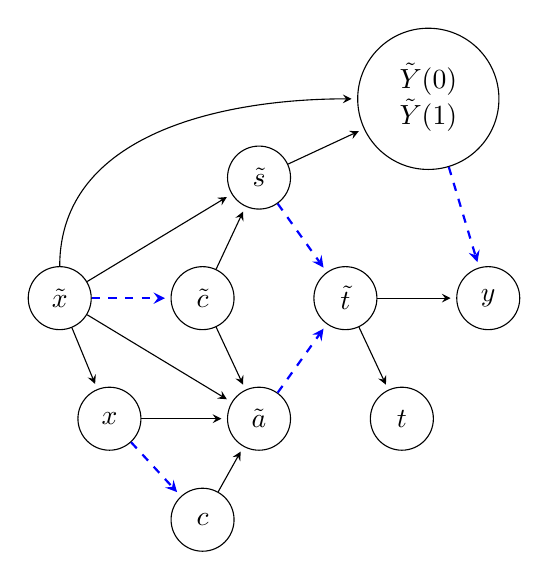
\begin{tikzpicture}[%
->,
shorten >=2pt,
>=stealth,
node distance=1cm,
pil/.style={
->,
thick,
shorten =2pt,}
]
\node[circle, draw, minimum size=0.80cm] (Xt) {$\tilde{x}$};
\node[circle, draw, minimum size=0.80cm] [right= of Xt] (Ct) {$\tilde{c}$};
\node[circle, draw, minimum size=0.80cm] [below=2 of Ct] (C) {$c$};
\node[above= of Xt] (AXt) {};
\node[below= of Xt] (BXt) {};
\node[circle, draw, minimum size=0.80cm] [right=0.1 of BXt] (X) {$x$};
\node[circle, draw, minimum size=0.80cm] [right=2 of BXt] (at) {$\tilde{a}$};
\node[circle, draw, minimum size=0.80cm] [right=2 of AXt] (St) {$\tilde{s}$};
\node[circle, draw, minimum size=0.80cm] [right= of Ct] (tt) {$\tilde{t}$};
\node[circle, draw, minimum size=0.80cm] [right= of at] (t){$t$};
\node[above=2 of tt] (Att){};
\node[circle, draw, minimum size=0.80cm] [right=.025 of Att] (Yt)
{\begin{tabular}{c}$\tilde{Y}(0)$\\
$\tilde{Y}(1)$\end{tabular}};
\node[circle, draw, minimum size=0.80cm] [right= of tt] (y) {$y$};

\draw[->] (Xt) --(X);
\draw[->, color=blue, thick, dashed] (Xt) --(Ct);
\draw[->, color=blue, thick, dashed] (X) --(C);
\draw[->] (Xt) --(at);
\draw[->] (Ct) --(at);
\draw[->] (C) --(at);
\draw[->] (X) --(at);
\draw[->] (Xt) --(St);
\draw[->] (Ct) --(St);
\draw[->, color=blue, thick, dashed] (St) --(tt);
\draw[->, color=blue, thick, dashed] (at) --(tt);
\draw[->] (tt) --(t);
\draw[->] (St) --(Yt);
%\draw[->] (at) --(Yt);
%\draw[->] (Xt) --(Yt);
\draw[->, color=blue, thick, dashed] (Yt) --(y);
\draw[->] (tt) --(y);
\draw[->] (Xt) to [out=90,in=180] (Yt);
%\draw[->] (1) to [out=150,in=165] (4);
\end{tikzpicture}
\end{figure}

\end{frame}

\begin{frame}
\frametitle{Evaluating the NSLP -- Sketch of a Larger Model}
Starting with the threshold covariate:
\begin{align*}
\tilde{x}_i\stackrel{ind}{\sim} N(\bm{z}_i'\bm{\beta}_{\tilde{x}},\sigma_{\tilde{x}}^2)&&\mbox{and}&&x_i\stackrel{ind}{\sim} N(\tilde{x}_i,\sigma_{x}^2)
\end{align*}

\pause Let
\begin{align*}
\tilde{a}_i=\indicator{a^*_i>0} &&\mbox{and}&&\tilde{s}_i=\indicator{s^*_i>0}
\end{align*}
where
\begin{align*}
a_i^*\stackrel{ind}{\sim} & N(\bm{z}_i'\bm{\beta}_{a^*} +
\tilde{c}_i\lambda_{a^*} + c_i\gamma_{a^*} + \tilde{x}_i\theta_{a^*} +
x_i\phi_{a^*}, 1)\\
s_i^*\stackrel{ind}{\sim} & N(\bm{z}_i'\bm{\beta}_{s^*} +
\tilde{c}_i\lambda_{s^*} + \tilde{x}_i\theta_{s^*} , 1)\\
\end{align*}
Then $\tilde{t}_i=\tilde{a}_i\tilde{s}_i$ \pause and let
\begin{align*}
t_i | \tilde{t}_i=0 \stackrel{ind}{\sim} & Ber(p)\\
t_i | \tilde{t}_i=1 \stackrel{ind}{\sim} & Ber(1-q)
\end{align*}
where $p$ is the false positive rate and $q$ is the false negative
rate. 
\end{frame}

\begin{frame}
\frametitle{Evaluating the NSLP -- Sketch of a Larger Model}
Define $Y^*_i(0)$ and $Y^*_i(1)$ such that $\tilde{Y}_i(k)=\indicator{Y^*_i(k)>0}$ where 
\[
\begin{bmatrix} Y_i^*(0) \\ Y_i^*(1) \end{bmatrix}
\stackrel{ind}{\sim} N \left( \begin{bmatrix}
    \bm{z}_i'\bm{\beta}_{y^*} + \tilde{x}_i\theta_{y^*} +
    s^*_i\psi_{y_0^*} \\
    \bm{z}_i'\bm{\beta}_{y^*} + \tilde{x}_i\theta_{y^*} +
    s^*_i\psi_{y_1^*} \end{bmatrix},
\begin{bmatrix}1 & \rho \\ \rho & 1 \end{bmatrix} \right)
\]
and $y_i=\tilde{Y}_i(\tilde{t}_i)$.\\~

$Y_i^*(k)$ represents an unobserved continuous measure of food security in counterfactual $k$.

\end{frame}

\begin{frame}
\frametitle{Evaluating the NSLP -- Large Model Identification Heuristics}
$\sigma_x^2$ and $\sigma_{\tilde{x}}^2$ both unidentified, but $\sigma_x^2 + \sigma_{\tilde{x}}^2$ is identified. \pause If 
\begin{align*}
Corr(x,\tilde{x}|\bm{z})>K&&\mbox{or equivalently}&&\frac{\sigma_x^2}{\sigma_x^2 + \sigma_{\tilde{x}}^2} > K^2
\end{align*}
then we can learn about both $\sigma_x^2$ and $\sigma_{\tilde{x}}^2$. \\~\\

\pause To learn about the components of the $a_i^*$ and $s_i^*$ equations, we need to learn about $a_i^*$ and $s_i^*$ $\implies$ need to learn about $p$ and $q$. \pause If $p + q > 1$ in the prior then we can learn about $p$, $q$, and $\tilde{t}_i$.\\~\\

\pause When $\tilde{t}_i=1$ we know $\tilde{a}_i=\tilde{s}_i=1$ which lets us update our priors on the parameters in the $a^*_i$ and $s_i^*$ equations.\\~\\

\pause $\rho=Corr(Y^*(0),Y^*(1)|s^*)$ is also unidentified.\\
\pause\ \ $\implies$ can learn about $E[TE|y]$ but maybe not about $p(TE|y)$...\\
\pause But we do learn about $Corr(Y^*(0),Y^*(1)|\tilde{x},\bm{z})$ through positive definite restrictions $\implies$ learning about $p(TE|y)$.

\end{frame}

\begin{frame}
\frametitle{Evaluating the NSLP -- Open Questions for the Large Model}
\begin{enumerate}
\item Priors that acknowledge that households near the income cutoff but on opposite sides are similar.
\item Use outside information of classification error rates in the priors.
\item Check whether partial identification heuristics are correct.
\item Nonparametric link functions.
\item Nonparametric
\item Alternative specifications.
\item Still need to take into account the survey weights.
\end{enumerate}
\end{frame}

\bibliographystyle{plainnat}
\bibliography{../dlmasis/doc/dlmasis}


\end{document}

